\chapter{Technical Solution}

\section{Set up}
Since I am developing a dynamic website, using javascript modules is against the CORS policy,
\footnote{https://stackoverflow.com/questions/52919331/access-to-script-at-from-origin-null-has-been-blocked-by-cors-policy}
therefore I have decided to use an npm (javascript package manager) package\footnote{https://www.npmjs.com/package/live-server/v/0.8.0} \verb|live-server| to host my website on a live server.
It is a command line application, and when ran using \verb|live-server| simply searches for an \verb|index.html| file and hosts it using an IP address with a port. By default, it hosts on \verb|localhost:8080|, allowing for easy debugging of your web page. \\
Firstly, let's create a simple project structure to host our project. Initially, I created a basic \verb|index.html| file. Since most of our graphical interface will be written in javascript, all I have to specify is the import of the actual javascript file, and some extra tags. \\
The \verb|<script type="module" src="js/main.js">| tag imports the \verb|main.js| file in the \verb|js| folder. \\
I set the title of the project as seen by this line: \verb|<title>Globe</title>|, and then disabled any sort of margin on our page by the CSS within the \verb|<style>| tags.
\newpage
\textbf{index.html}
\begin{lstlisting}[language=Html]
<!DOCTYPE html>
<html>
	<head>
		<meta charset="utf-8">
		<title>Globe</title>
		<style>
			body { margin: 0; }
		</style>
	</head>
	<body>
    	<script type="module" src="js/main.js"></script>
	</body>
</html>
\end{lstlisting}

\dotfill

\textbf{js/main.js}
\begin{lstlisting}
console.log("Hello world");
\end{lstlisting}

\dotfill

After running \verb|live-server|, the output in the web browser is: \\
\begin{figure}[h]
\centering
\includegraphics[width=0.7\linewidth]{images/setup_output}
\caption{}
\label{fig:setupoutput}
\end{figure}

\newpage

\section{THREE.js}
Now that I have set up a basic frame upon which to build our application on, we need to import \verb|THREE.js|, the graphical framework we will be using referenced in the Analysis section. \verb|THREE.js| is, fortunately, very simple to set up. All we need to do is import the javascript file in our \verb|main.js| file. Since \verb|main.js| is a module, we can easily import other javascript modules from the javascript file. However, before importing the file, we need to install the \verb|THREE.js| library. Since it's a single-file library, all we need to do is navigate to their website\footnote{https://threejs.org} and click the \verb|download| button, and import the file downloaded. \\
It's easy to import files in javascript, this is our javascript file currently: \\


\textbf{js/main.js}
\begin{lstlisting}
import * as THREE from "./three.js";
console.log("Hello world");
\end{lstlisting}
As an overview, the \verb|import| statement allows for importing files, we use the \verb|*| wildcard to import \textbf{everything} from \verb|three.js| and alias it under a namespace \verb|THREE|. Code further ahead will use this namespace. \\
We get the same output, and we get no errors, which means that \verb|THREE.js| has been imported successfully.

\newpage

\subsection{Setting up the scene}\footnote{https://threejs.org/docs/index.html\#manual/en/introduction/Creating-a-scene}
The goal of this section is to set up the scene for our globe page, as a brief example, I will create a spinning sphere as the basis for our graphical web page. Firstly, let's actually \textit{create} the scene:

\begin{lstlisting}
const scene = new THREE.Scene();
const camera = new THREE.PerspectiveCamera(75, window.innerWidth / window.innerHeight, 0.1, 1000);

const renderer = new THREE.WebGLRenderer();
renderer.setSize(window.innerWidth, window.innerHeight);
document.body.appendChild(renderer.domElement);
\end{lstlisting}

The \verb|scene| variable, contains information in regards to the actual \textit{scene}. \\
Since we are looking at our globe from a perspective, we initialize the \verb|THREE| class \verb|PerspectiveCamera|. \\ The first parameter is the \textit{field of view}, the extent of the scene which can be seen on display at any moment. I set it to $75^{\circ}$. \\
The second parameter is the \textit{aspect ratio}, which determines how wide the pixels are on the screen. For mostly all monitors, the aspect ratio is defined:
\begin{align*}
Aspect\ Ratio = \frac{Window\ Width}{Window\ Height}
\end{align*}
The fact that \verb|window.innerWidth| or \verb|window.innerHeight| are variable, means that as the window is resized, so will the scene. \\
The next two parameters are the \verb|near| and \verb|far| clipping plane. Which creates a interval at which objects won't be rendered. For example, objects further than \verb|far| will not render, and objects closer than \verb|near| will also not render. For now, I don't exactly know how big the globe will be, and so I used arbitrary values $0.1$ and $1000$ for \verb|near| and \verb|far| respectively. \\

Now, we need to define a renderer to render the scene. \verb|THREE.js| comes with many renderers, however I chose to use the most conventional renderer, the \verb|WebGLRenderer| class. It uses WebGL, a web version of OpenGL, to render objects. I want the renderer to fill the entire screen, and so I chose for it to render at maximum width and height. \\
Finally, we want to add the renderer to our HTML document. Behind the scenes, \verb|THREE.js| uses a \verb|<canvas>| tag to render everything.

\newpage
\subsection{Populating the scene}\footnote{https://threejs.org/docs/index.html\#manual/en/introduction/Creating-a-scene}
Now that we have created a scene, let's define some objects to populate the scene. I am going to populate the scene with a spinning sphere. \verb|THREE.js| makes this task very simple:
\begin{lstlisting}
const geometry = new THREE.SphereGeometry(5);
const material = new THREE.MeshBasicMaterial({color: 0xff0000});
const sphere = new THREE.Mesh(geometry, material);
scene.add(sphere);

camera.position.z = 10;
\end{lstlisting}
The \verb|geometry| variable contains all the vertices and faces of the sphere. \verb|THREE.js| has many simple shape geometries that can easily be created, and for this case we need a sphere, so we use the \verb|SphereGeometry| class with initial radius of $5$. \\
The \verb|material| variable apply properties to a certain geometry, and allows us to colour the faces of our sphere with any colour of our liking, as well as allow for more complex materials such as images. \verb|MeshBasicMaterial| is a basic interface class which allows us to specify basic properties. I want the sphere to be red, and so we pass an empty table to \verb|MeshBasicMaterial| with an attribute \verb|color| that contains a hex colour \verb|0xff0000|. Hex colours work by dividing a 24 bit number into 3 parts, the red, the green, and the blue parts. Each part can have a range from 0-255 e.g \verb|0xff = 255|. For our sphere to render in red, we want to only colour the red part of the hex colour. If we split up our hex colour it would look like this:
\begin{center}
\begin{tabular}{|c| |c| |c|}
FF & 00 & 00 \\
R  & G  & B
\end{tabular}
\end{center}
Now we can actually create the object. Objects in \verb|THREE.js| are called 'Meshes'. The \verb|sphere| variable contains a mesh taking our \verb|geometry| variable and our \verb|material| variable respectively. The reason we define the geometry and material variables is so that we can modify them later when we want to animate our sphere. \\
Finally, we add the sphere to the scene. However, since the camera is placed at \verb|(0, 0, 0)|, we want to shift the camera backwards so that we can actually \textit{see} the sphere. I moved it to the point \verb|(0, 0, 10)| by changing \verb|camera.position.z| to $10$. \\
However, we are still not done yet, since we have to render and animate our scene.

\newpage
\subsection{Rendering and animating the scene}\footnote{https://threejs.org/docs/index.html\#manual/en/introduction/Creating-a-scene}
Now, we can finally render our scene. \verb|THREE.js| makes this task simple and quick. Conventionally, we define a function \verb|animate| which will contain all the code we wish to repeat in the program loop. This is how we do this:
\begin{lstlisting}
function animate() {
  requestAnimationFrame(animate);
  renderer.render(scene, camera);
}
animate();
\end{lstlisting}
The \verb|animate| function creates an infinite loop which redraws the scene every time the \textit{screen} is refreshed, usually 60 times per second. The \\ \verb|requestAnimationFrame| function takes in the \verb|animate| function and actually creates this loop, which is a nice abstraction. \\
Then the renderer renders our scene with our camera, and finally, we call the \verb|animate| function to actually run this snippet of code.
\begin{figure}[h]
\centering
\includegraphics[width=0.7\linewidth]{images/setup_output2}
\caption{}
\label{fig:setupoutput2}
\end{figure}

Finally, our sphere can be seen on the screen! However, we have created no way for it to rotate. \\
Note that our \verb|animate| function gets called 60 times per second. This is where we want to place our rotation code. \\
\newpage
Here's our updated \verb|animate| function:
\begin{lstlisting}
function animate() {
  sphere.rotateY(0.01);

  requestAnimationFrame(animate);
  renderer.render(scene, camera);
}
animate();
\end{lstlisting}
\verb|sphere.rotateY(0.01)| rotates the sphere in the y axis by $0.01$ radians every $\frac{1}{60}$th of a second. \verb|THREE.js| rotations look like this:
\begin{figure}[h]
\centering
\includegraphics[width=0.3\linewidth]{images/setup_output4}
\caption{}
\label{fig:setupoutput4}
\end{figure}\footnote{https://cdn.kastatic.org/ka-perseus-images/d24dd08a0ea7aaeeaa90d84f642e12998df3ffe7.svg}

It's quite hard to see on the screen due to the fact the sphere is one solid colour, however we can set the \verb|wireframe| attribute in the \verb|MeshBasicMaterial| class to true like so. It allows us to see only the outlines of the sphere:
\begin{lstlisting}
const material = new THREE.MeshBasicMaterial({
	color: 0xff0000, 
	wireframe: true
});
\end{lstlisting}
Our sphere now rotates anti-clockwise on the y axis, and looks like this:
\begin{figure}[h]
\centering
\includegraphics[width=0.5\linewidth]{images/setup_output3}
\caption{}
\label{fig:setupoutput3}
\end{figure}

\subsection{Overview}
\textbf{index.html}
\begin{lstlisting}[language=Html]
<!DOCTYPE html>
<html>
	<head>
		<meta charset="utf-8">
		<title>Globe</title>
		<style>
			body { margin: 0; }
		</style>
	</head>
	<body>
    <script type="module" src="js/main.js"></script>
	</body>
</html>
\end{lstlisting}
\newpage
\textbf{js/main.js}
\begin{lstlisting}
import * as THREE from './three.js';

const scene = new THREE.Scene();
const camera = new THREE.PerspectiveCamera(75, window.innerWidth / window.innerHeight, 0.1, 1000);

const renderer = new THREE.WebGLRenderer();
renderer.setSize(window.innerWidth, window.innerHeight);
document.body.appendChild(renderer.domElement);

const geometry = new THREE.SphereGeometry(5);
const material = new THREE.MeshBasicMaterial({color: 0xff0000, wireframe: true});
const sphere = new THREE.Mesh(geometry, material);
scene.add(sphere);

camera.position.z = 10;

function animate() {
  sphere.rotateY(0.01);

  requestAnimationFrame(animate);
  renderer.render(scene, camera);
}

animate();
\end{lstlisting}
\newpage






\section{WebGL Shaders and GLSL}
WebGL is the way \verb|THREE.js| interacts with graphics. We enabled WebGL rendering earlier by setting our \verb|renderer| to a \verb|THREE.WebGLRenderer|. It allows for graphics to be ran on the GPU instead of the CPU, allowing for huge performance boosts over CPU drawing. In essence, WebGL is a javascript API to allow users to draw graphics on the screen with maximum performance. Performance is important because if we want to draw a complex scene 60 times per second, we need to be performant. \\
The reason we need to worry about this, is that for us users to create beautiful graphical effects efficiently is to communicate with the WebGL \textit{shader pipeline}.
\subsection{Introduction to shaders}\footnote{https://learnopengl.com/Getting-started/Shaders}
Now that we have created our sphere, I think it's time to turn it into a globe. To do this, we need to introduce shaders. \\
Shaders are little programs that \textbf{rest on the GPU}. They belong in a \textit{shader pipeline}.
\footnote{https://www.khronos.org/opengl/wiki/Rendering\_Pipeline\_Overview}. \\
The shader pipeline is a sequence of steps that WebGL takes when rendering objects. It consists of many steps, but to keep it simple, we will focus on two important steps which we can manipulate: vertex processing and fragment processing. \\
The way we render positions in WebGL is by taking many vertices and processing them, for example, a cube has 8 vertices, each with a position. A 1x1 cube may be defined like this in WebGL: \\
\begin{center}
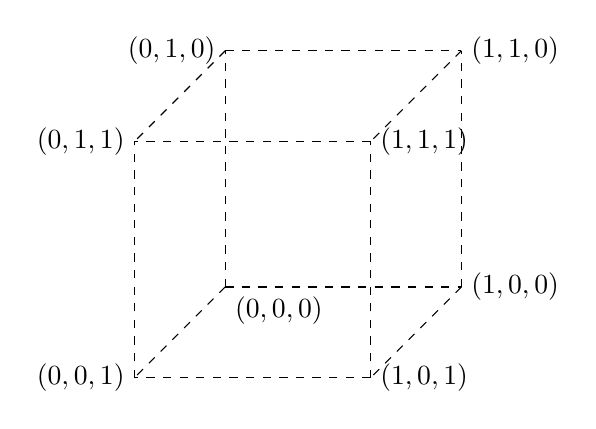
\begin{tikzpicture}
	\coordinate (A1) at (0, 0, 0);
	\coordinate (A2) at (3, 0, 0);
	\coordinate (A3) at (0, 0, 3);
	\coordinate (A4) at (3, 0, 3);
	\coordinate (B1) at (0, 3, 0);
	\coordinate (B2) at (3, 3, 0);
	\coordinate (B3) at (0, 3, 3);
	\coordinate (B4) at (3, 3, 3);
	
	\node[below right] at (A1) {$(0, 0, 0)$};
	\node[right] at (A2) {$(1, 0, 0)$};
	\node[left] at (A3) {$(0, 0, 1)$};
	\node[right] at (A4) {$(1, 0, 1)$};
	\node[left] at (B1) {$(0, 1, 0)$};
	\node[right] at (B2) {$(1, 1, 0)$};
	\node[left] at (B3) {$(0, 1, 1)$};
	\node[right] at (B4) {$(1, 1, 1)$};
	
	\draw[dashed] (A1) -- (A2);
	\draw[dashed] (A2) -- (A4);
	\draw[dashed] (A4) -- (A3);
	\draw[dashed] (A1) -- (A3);
	
	\draw[dashed] (B1) -- (B2);
	\draw[dashed] (B2) -- (B4);
	\draw[dashed] (B4) -- (B3);
	\draw[dashed] (B1) -- (B3);
	
	\draw[dashed] (A1) -- (B1);
	\draw[dashed] (A2) -- (B2);
	\draw[dashed] (A3) -- (B3);
	\draw[dashed] (A4) -- (B4);
\end{tikzpicture}
\end{center}

A vertex shader, therefore, performs manipulations on these coordinates.
\newpage
A fragment shader, acts not on the coordinates, but on \verb|fragments|\footnote{https://www.khronos.org/opengl/wiki/Fragment}. A \verb|fragment| is a collection of values, each representing a segment of an area of pixels. You can think of this as segments of the faces of the sphere. Therefore, a fragment shader is a little program to perform manipulations on the pixels themselves. This allows us to, for example, change the colour of the pixels themselves depending on the vertex of the object. \\
These are combined into a \textit{shader pipeline}, where the vertex shader program is ran, then its output is \textit{piped} into the fragment shader program. \\
GLSL\footnote{https://www.khronos.org/opengl/wiki/OpenGL\_Shading\_Language} is the programming language in which we will write our shaders in. It's a C-style language, and is specifically designed for vertex/fragment shaders.

\subsection{Shading}
Let's convert our sphere from a \verb|MeshBasicMaterial| to a \verb|ShaderMaterial|. A \verb|ShaderMaterial| allows us to add a shader to our object. \\
Firstly, I changed our \verb|material| variable to:
\begin{lstlisting}
const material = new THREE.ShaderMaterial({
	uniforms: {
		time: clock.getElapsedTime()
	},
	
	vertexShader: sphereShader.vertex,
	fragmentShader: sphereShader.fragment,
});
\end{lstlisting}
Let's take a moment to understand these changes, the \verb|uniforms| attribute lets us pass in values from our javascript program to our shader files. That's what a uniform is, a sort of 'parameter' into the shader. \\
Now, we pass our user defined shaders into the \verb|vertexShader| and \verb|fragmentShader| attributes. We actually haven't defined \verb|sphereShader|. Let's define this in a new file \verb|shader/sphereShader.js|.
\newpage
\textbf{shader/sphereShader.js}
\begin{lstlisting}
export const vertex = ``;

export const fragment = ``;
\end{lstlisting}
We will write our vertex shader in the \verb|vertex| variable, and the fragment shader in the \verb|fragment| variable.
Now, we have some shaders. Let's try to open the webpage.
\begin{figure}[h]
\centering
\includegraphics[width=0.7\linewidth]{images/shader_output1}
\caption{}
\label{fig:shaderoutput1}
\end{figure} \\
We've ran into a problem. WebGL is telling us that our vertex shader has no \verb|main()| function. The way GLSL works is that when a shader gets executed, WebGL calls the \verb|main()| function, where all the calculations and manipulations are made. Let's define it for both shaders.
\begin{lstlisting}
export const vertex = `void main(void) { }`;

export const fragment = `void main(void) { }`;
\end{lstlisting}
We define functions in GLSL like \verb|type function_name(types...) { ... }|. The type of \verb|main(void)| is \verb|void|, which means the function does not return anything. If we were to define a function like \verb|int foo(...) { return x; }|, x must be of an int type. \\
Let's open our page again.
\begin{figure}[h]
\centering
\includegraphics[width=0.7\linewidth]{images/shader_output2}
\caption{}
\label{fig:shaderoutput2}
\end{figure} \\
We get another error! The error describes us as not having any shader outputs. This is because both shaders, vertex and fragment must output something. In WebGL, the output variable is called \verb|gl_Position| for vertex shaders and \verb|gl_FragColor| for fragment shaders. With this information, let's try and draw our sphere again.
\newpage
Let's begin with the vertex shader. Recall that the vertex shader takes many vertices and performs calculations on these vertices so that they 'project' onto our screen. After some testing, this is what I came up with:
\begin{lstlisting}
varying vec3 vUv;
void main(void) {
  vUv = position;

  vec4 modelViewPosition = modelViewMatrix * vec4(position, 1.0);
  gl_Position = projectionMatrix * modelViewPosition;
}
\end{lstlisting}
Let's break this down. Firstly, we define a global \verb|varying vec3 vUv|. The \verb|varying| tags the \verb|vec3 vUv| as being part of the pipeline. This means that this variable \verb|vUv| will be passed onto the next shader (the fragment shader). \\
\verb|vUv| is shorthand for the \textit{coordinate of the vertex}, it will be useful later when we use it in the fragment shader. \\
After the \verb|main(void)| definition, we set \verb|vUv| as the \verb|position| global, where \verb|position| is the position of the vertex. \\
\verb|modelViewMatrix| is a global 4D matrix (\verb|mat4|) which contains all transformations, rotations and scaling required to put a vertex in its position.
\footnote{http://www.opengl-tutorial.org/beginners-tutorials/tutorial-3-matrices/} \\
With this information, we know that we have to translate the vertex by the translation matrix. This is what an example \verb|modelViewMatrix| looks like:
\begin{align*}
modelViewMatrix = 
\begin{bmatrix}
... & ... & ... & v_{x} \\
... & ... & ... & v_{y} \\
... & ... & ... & v_{z} \\
... & ... & ... & 1.0
\end{bmatrix}
\end{align*}
Where $v_{n}$ is the position of the vertex in \textbf{relation to the model}. Because this matrix is relative, we need to turn it into a real world position on the screen. Therefore, we need to translate our existing \verb|position| by the \verb|modelViewMatrix|:
\begin{align*}
modelViewPosition = modelViewMatrix *
\begin{bmatrix}
p_{x} \\ p_{y} \\ p_{z} \\ 1
\end{bmatrix}
\end{align*}
Where $p_{n}$ is the coordinate of the 3D vector WebGL \verb|position|.
\newpage
Finally, we further translate our position by the \verb|projectionMatrix|. Since we view the program through a 'camera', we need to further translate the real world position into a position that correlates to the screen. In other words, a vertex that happens to have $x = 0$ and $y = 0$ should be rendered at the center of the screen. However, it's not as simple as the $x$ and $y$ coordinates, since we are rendering 3D, the $z$ coordinate also counts. For two vertices with $v1_{x} = v2_{x}$ and $v1_{y} = v2_{y}$, the vertex with the biggest $z$ coordinate will be \textbf{more on the center of the screen than another}, just like how we \textit{see} in perspective. To do this, we just transform it again:
\begin{align*}
finalPosition = projectionMatrix * modelViewPosition
\end{align*}
Here is a way to visualize it. We have blue objects in the scene, and the red shape represents the frustum of the camera - \textit{the part of the scene the camera can actually see.}
\begin{figure}[h]
\centering
\includegraphics[width=0.5\linewidth]{images/shader_output3}
\caption{}
\label{fig:shaderoutput3}
\end{figure} \\
When we multiply \textbf{everything} by the projection matrix (i.e everything is the \verb|modelViewPosition|) it has the following effect:
\begin{figure}[h]
\centering
\includegraphics[width=0.5\linewidth]{images/shader_output4}
\caption{}
\label{fig:shaderoutput4}
\end{figure} \\
Now the projection looks like a cube, and from 'behind' the camera frustum it looks like this:
\begin{figure}
\centering
\includegraphics[width=0.5\linewidth]{images/shader_output6}
\caption{}
\label{fig:shaderoutput6}
\end{figure} \\
\begin{footnotesize}
Images taken from http://www.opengl-tutorial.org/beginners-tutorials/tutorial-3-matrices/
\end{footnotesize}

The reason that WebGL uses matrices for translations, rotations and scaling is that matrices are a singular structure. This means that we can move around all this information in just a single structure.

\newpage
\subsection{Mapping the globe texture}
Instead of using a \verb|ShaderMaterial| for our sphere, I will switch back to a \verb|MeshBasicMaterial|. \verb|THREE.js| allows us to easily map a texture using a \verb|TextureLoader|. I saved the texture in a new folder \verb|texture|.\footnote{Texture: https://www.solarsystemscope.com/textures/}

\begin{lstlisting}
const texture = new THREE.TextureLoader().load('texture/8k_earth_daymap.jpg')
const material = new THREE.MeshBasicMaterial({
    map: texture
})
\end{lstlisting}

Now that our material has been changed, updating our project, our globe looks like this: \\
\begin{figure}[ht]
\centering
\includegraphics[width=0.5\linewidth]{images/mapping}
\caption{}
\label{fig:mapping}
\end{figure}
\\ This is quite an ugly looking planet however, and so I decided to create an atmosphere.
\newpage
\subsection{Creating an atmosphere}
An atmosphere can be created by adding another, slightly larger, sphere to the scene. Since our planet has a radius of 5, I chose to let the atmosphere's radius to be 5.02. The atmosphere will be a good example of usage of \verb|GLSL|. \\
Firstly, we need to create the atmosphere sphere, this is exactly the same as the globe, however, instead of the \verb|MeshBasicMaterial|, we will use a \verb|ShaderMaterial|:
\begin{lstlisting}
import * as sphereShader from "./shader/sphereShader.js";

const atmosphere = new THREE.Mesh(
    new THREE.SphereGeometry(5.02, 64, 64),
    new THREE.ShaderMaterial({
        transparent: true,
        vertexShader: sphereShader.vertex,
        fragmentShader: sphereShader.fragment,
    })
);
\end{lstlisting}
Now, we need to define our atmosphere shader \verb|sphereShader|. This is defined in a different file located in "shader/sphereShader.js".
Looking back at our atmosphere algorithm:
\begin{lstlisting}
Intensity = DotProduct(Normal, Vector(0, 0, 1))
Atmosphere = Vector(0, 1.2, 2.0) * Intensity
Pixel Colour = Vector(Atmosphere.XYZ, 0.5)
\end{lstlisting}
We need to translate this pseudocode into actual GLSL code: \\
\newpage
\textbf{Vertex Shader}
\begin{lstlisting}
varying vec3 vUv;
varying vec3 vNormal;
void main(void) {
  vUv = position;

  vec4 modelViewPosition = modelViewMatrix * vec4(position, 1.0);
  gl_Position = projectionMatrix * modelViewPosition;
  vNormal = normalize(normalMatrix * normal);
}
\end{lstlisting}

\textbf{Fragment Shader}
\begin{lstlisting}
varying vec3 vUv;
varying vec3 vNormal;

void main(void) {
  float intensity = 1.25 - dot(vNormal, vec3(0.0, 0.0, 1.0));
  vec3 atmosphere = vec3(1.0, 1.0, 1.0) * pow(intensity * 1.5, 3.0);
  gl_FragColor = vec4(vec3(0.0, 0.7, 2.0) * atmosphere, 0.5);
}
\end{lstlisting}
After tweaking some parameters, our \verb|GLSL| code is not quite the same as our pseudocode. Firstly, I clamped the \verb|Intensity| to be at \textbf{least} 1.25, otherwise our atmosphere will be too thin. After that, I modified the \verb|atmosphere| vector to follow this formula: \\
$$\textrm{Atmosphere} = \begin{bmatrix}1 \\ 1 \\ 1\end{bmatrix} \cdot (1.5\textrm{Intensity})^2$$
\newpage
The singleton vector of 1 essentially turns our intensity variable into a \verb|vec3|, and I further tweaked the intensity so that the further the pixel is from the center, the less opaque it is. Finally, I multiplied the finalized atmosphere vector with a cyan-ish colour, and toned down the final opacity of the globe to $0.5$. After adding the \verb|atmosphere| mesh to the scene (\verb|scene.add(atmosphere)|) our globe looks like this: \\
\begin{figure}[ht]
\centering
\includegraphics[width=0.5\linewidth]{images/atmosphere}
\caption{}
\label{fig:atmosphere}
\end{figure}
\\
I think it still looks a bit lacklustre, and so I've decided to add some stars to the background.

\subsection{Stars}
I want a lot of stars in the background, however, I think that adding each star as a \verb|SphereGeometry| would slow down the project a lot. I want thousands of stars, and I don't think each star needs to be a sphere, instead we can dumb down each star to represent a single pixel. In \verb|THREE.js| we have access to a data structure called a \verb|BufferGeometry|. A \verb|BufferGeometry| stores a constant amount of 'vertices', very efficiently. Since I only need stars to be pixels, I can just represent them as points, thus \verb|BufferGeometry| is a perfect fit for this, as it only stores coordinates (vertices). \\
\newpage
Firstly, lets create an array containing a large amount of x,y,z coordinates.
\begin{lstlisting}
const star_vertices = [];
for (let i = 0; i < 10000; i++) {
    const x = THREE.MathUtils.randFloatSpread(2000);
    const y = THREE.MathUtils.randFloatSpread(2000);
    const z = THREE.MathUtils.randFloatSpread(2000);

    star_vertices.push(x,y,z);
}
\end{lstlisting}
Here I create 10000 random x,y,z coordinates with each coordinate spread in a range of 0 to 2000 using the \verb|randFloatSpread| function.

Now, we convert this array into a \verb|BufferGeometry| as such:
\begin{lstlisting}
const star_geometry = new THREE.BufferGeometry();
star_geometry.setAttribute('position', new THREE.Float32BufferAttribute(star_vertices, 3));
\end{lstlisting}

Let's convert this into a mesh, using a \verb|ShaderMaterial| as the material, and \verb|Points| as the mesh. The \verb|Points| mesh just holds vertices, just like the \verb|BufferGeometry|.
\begin{lstlisting}
import * as starShader from "./shader/starShader.js";

const star_material = new THREE.ShaderMaterial({ 
    uniforms: star_uniforms,
    vertexShader: starShader.vertex,
    fragmentShader: starShader.fragment,
});
const stars = new THREE.Points(star_geometry, star_material);
\end{lstlisting}
\newpage
Let's also create a \verb|GLSL| shader pipeline for the stars \verb|starShader|, we will leave the vertex shader as normal without any vertex manipulation, since we will only manipulate the fragment shader. \\
\textbf{Fragment Shader}
\begin{lstlisting}
varying vec3 vUv;
varying vec3 vNormal;

uniform float delta;

void main(void) {
    vec3 vN = normalize(vUv);
    vec3 blink = vec3(1.0, 1.0, 1.0) * sin(delta * 0.05 + vUv.x);
    gl_FragColor = vec4(blink, 1.0);
}
\end{lstlisting}
The fragment shader simply adds a flicker to each star, over time (\verb|delta|). Firstly, I normalized the vertex position (\verb|vUv|) to reduce the large position range into a decimal number from 0 to 1. Secondly, I added a flicker to the stars (\verb|blink|) by multiplying the color white \verb|vec3(1.0, 1.0, 1.0)| with a slowly changing sine wave \verb|sin(delta * 0.05 + vUv.x)|.
\begin{figure}[ht]
\centering
\includegraphics[width=0.5\linewidth]{images/stars}
\caption{}
\label{fig:stars}
\end{figure}
\newpage
\subsection{Overview}
No changes made to \verb|index.html|. \\

Changes made to \verb|main.js|:
\begin{lstlisting}
import * as sphereShader from "./shader/sphereShader.js";
import * as starShader from "./shader/starShader.js";

// Create globe object
const geometry = new THREE.SphereGeometry(5, 64, 64);
const texture = new THREE.TextureLoader().load('texture/8k_earth_daymap.jpg');

const material = new THREE.MeshBasicMaterial({
  map: texture
});
const sphere = new THREE.Mesh(geometry, material);
scene.add(sphere);

// Create atmosphere object
const atmosphere = new THREE.Mesh(
  new THREE.SphereGeometry(5.02, 64, 64),
  new THREE.ShaderMaterial({
    transparent: true,
    vertexShader: sphereShader.vertex,
    fragmentShader: sphereShader.fragment,
  })
);

scene.add(atmosphere);

// Create stars
const star_vertices = [];
for (let i = 0; i < 10000; i++) {
    const x = THREE.MathUtils.randFloatSpread(2000);
    const y = THREE.MathUtils.randFloatSpread(2000);
    const z = THREE.MathUtils.randFloatSpread(2000);

    star_vertices.push(x,y,z);
}

const star_geometry = new THREE.BufferGeometry();
star_geometry.setAttribute('position', new THREE.Float32BufferAttribute(star_vertices, 3));

// The delta uniform is modified every animation tick
// We can use the delta uniform in the star shader to cause blinking of the stars
let star_uniforms = {
    delta: { value: 1.0 },
};

const star_material = new THREE.ShaderMaterial({ 
    uniforms: star_uniforms,
    vertexShader: starShader.vertex,
    fragmentShader: starShader.fragment,
});
const stars = new THREE.Points(star_geometry, star_material);
scene.add(stars);

function animate() {
  // Here I am updating the delta uniform so it increases by 0.5 every animation tick
  star_uniforms.delta.value += 0.5;

  requestAnimationFrame(animate);
  renderer.render(scene, camera);
}

animate();
\end{lstlisting}

\textbf{shader/sphereShader.js}
This is the shader code for the globe's atmosphere.
\begin{lstlisting}
export const vertex = `
varying vec3 vUv;
varying vec3 vNormal;
void main(void) {
  vUv = position;

  vec4 modelViewPosition = modelViewMatrix * vec4(position, 1.0);
  gl_Position = projectionMatrix * modelViewPosition;
  vNormal = normalize(normalMatrix * normal);
}
`;

export const fragment = `
varying vec3 vUv;
varying vec3 vNormal;

void main(void) {
  float intensity = 1.25 - dot(vNormal, vec3(0.0, 0.0, 1.0));
  vec3 atmosphere = vec3(1.0, 1.0, 1.0) * pow(intensity * 1.5, 3.0);
  gl_FragColor = vec4(vec3(0.0, 0.7, 2.0) * atmosphere, 0.5);
}
`;
\end{lstlisting}

\textbf{shader/starShader.js}
This is the shader code for the stars.
\begin{lstlisting}
export const vertex = `
varying vec3 vUv;
varying vec3 vNormal;
void main(void) {
  vUv = position;

  vec4 modelViewPosition = modelViewMatrix * vec4(position, 1.0);
  gl_Position = projectionMatrix * modelViewPosition;
  vNormal = normalize(normalMatrix * normal);
}
`;

export const fragment = `
varying vec3 vUv;
varying vec3 vNormal;

// Import delta uniform from star_uniforms
uniform float delta;

void main(void) {
    vec3 vN = normalize(vUv);
    vec3 blink = vec3(1.0, 1.0, 1.0) * sin(delta * 0.05 + vUv.x);
    gl_FragColor = vec4(blink, 1.0);
}
`;
\end{lstlisting}


\section{User Input}
\subsection{Orbital Controls}
Through my analysis, I have decided to control and rotate the globe using an orbital control system. \verb|THREE.js| supplies its own orbital control system. Since orbital control systems are quite complex, I have decided to go with \verb|THREE.js|'s version. My reasoning for this is that \verb|THREE.js|'s version is fast, small, and allows for a lot of functionality. \\
Firstly, I need to import the orbital control system, and attach it to our web app:
\begin{lstlisting}
import { OrbitControls } from './OrbitControls.js';
// Attach the controls to our camera and allow it to have access to the domElement for events
const controls = new OrbitControls(camera, renderer.domElement);
\end{lstlisting}
I can finally see the back of the globe.
\begin{figure}[h]
\centering
\includegraphics[width=0.3\linewidth]{images/back}
\caption{}
\label{fig:back}
\end{figure}
And even zoom out.
\begin{figure}[h]
\centering
\includegraphics[width=0.3\linewidth]{images/zoom}
\caption{}
\label{fig:zoom}
\end{figure}

\newpage

\subsection{Country Selection}
Now I have to handle the mouse click, and correctly select a country. I am going to go with the nearest neighbour algorithm for selecting a country. \\
I need to add a listener for the 'mousedown' event, to execute an event on click. I have decided to structure the mouse as a 2D \verb|THREE.js| vector.
\begin{lstlisting}
document.addEventListener('mousedown', onDocumentMouseDown, false);
let mouse = new THREE.Vector2();

function onDocumentMouseDown(event) {
    console.log("Clicked!");
}
\end{lstlisting}
Now, whenever I click the webpage, it responds with "Clicked!"
\begin{figure}[h]
\centering
\includegraphics[width=0.6\linewidth]{images/clicked}
\caption{}
\label{fig:clicked}
\end{figure}
\\ I can also read the mouse coordinates:
\begin{lstlisting}
document.addEventListener('mousedown', onDocumentMouseDown, false);
let mouse = new THREE.Vector2();

function onDocumentMouseDown(event) {
    mouse.x = (event.clientX / window.innerWidth) * 2 - 1;
    mouse.y = -(event.clientY / window.innerHeight) * 2 + 1;
    console.log({x: mouse.x, y: mouse.y});
}
\end{lstlisting}
Now, whenever the user clicks on the web page, it responds with the \textbf{normalized} mouse coordinates on the screen. These coordinates range from -1 to 1, and are easier to work with than window size based coordinates.
\begin{figure}[ht]
\centering
\includegraphics[width=0.7\linewidth]{images/coords}
\caption{}
\label{fig:coords}
\end{figure}
\\ Now that we have access to the normalized mouse coordinates, we need somehow detect that the user has clicked on the sphere, and where on the sphere the user clicked. This involves usage of a \verb|THREE.js| class called the \verb|Raycaster|. The raycaster sends a 'ray' in which whatever object it intersects, it records its intersection position.
\begin{lstlisting}
const raycaster = new THREE.Raycaster();

function onDocumentMouseDown(event) {
    mouse.x = (event.clientX / window.innerWidth) * 2 - 1;
    mouse.y = -(event.clientY / window.innerHeight) * 2 + 1;
    
    // Position the raycaster so that it is in the same position as the camera
    raycaster.setFromCamera(mouse, camera);

    // Send a ray from the raycaster and check if it intersects with any 'sphere's, in this case, it should only intersect the globe.
    let globe = raycaster.intersectObject(sphere);

    // Iterate through all the intersections, there should only be one intersection anyways, but just in case there were no intersections, the for loop is skipped.
    for (let i = 0; i < globe.length; i++) {
        // 'point' represents the intersection coordinates
        let point = globe[i].point;

        // 'norm' represents the normalized intersection coordinates, to be converted into latitude and longitude, since its algorithm requires it.
        let norm = new THREE.Vector3(point.x, point.y, point.z);

        // normalize 'norm'
        norm.normalize();
    }
}
\end{lstlisting}
After this change, when the user clicks, the correct, normalized coordinates of the exact position of the click in relation to the sphere is recorded. I can finally convert this into latitude and longitude, and begin to select a country:
\begin{lstlisting}
let latitude = Math.asin(norm.y) * (180.0 / Math.PI);
let longitude = Math.atan2(norm.z, norm.x) * (-180.0 / Math.PI);
console.log({latitude, longitude});
\end{lstlisting}
When the user clicks on the globe now, the console responds:
\begin{figure}[h]
\centering
\includegraphics[width=0.7\linewidth]{images/latlong}
\caption{}
\label{fig:latlong}
\end{figure}
\\ After these changes, we can begin to detect and select countries. Firstly, we need to retrieve some sort of file which contains a list of countries, with their respective name and latitude and longitude coordinates. \\
I got my file from this MIT Licensed github repository: https://github.com/eesur/country-codes-lat-long \\
Each data entry is formatted as such: \\
\begin{lstlisting}
{
  "country" : "Albania",
  "alpha2" : "AL",
  "alpha3" : "ALB",
  "numeric" : 8,
  "latitude" : 41,
  "longitude" : 20
},
\end{lstlisting}
Since we now have each piece of the puzzle, we can begin connecting each piece. Firstly, we need to apply our nearest neighbour algorithm to select the country which is nearest to the latitude and longitude location. I turned this json file into a js file since json is embeddable in js, and imported it into my main.js file:
\begin{lstlisting}
import { countries } from './countries.js';
\end{lstlisting}
Now I can apply the nearest neighbour algorithm:
\begin{lstlisting}
// Calculate the distance between two objects { longitude: ..., latitude: ... }
function distance(a, b) {
  // Pythagorean rule
  let dx = a.longitude - b.longitude;
  let dy = a.latitude  - b.latitude;
  return Math.sqrt(dx*dx + dy*dy)
}

let lng_lat = { longitude, latitude }

let closest =
    countries["ref_country_codes"] // our json file contains this as its initial key
    .reduce((a, b) => distance(a, lng_lat) < distance(b, lng_lat) ? a : b)
\end{lstlisting}
I have condensed the algorithm into an argument to the javascript \verb|reduce| function. I have some experience with javascript, and I think the \verb|reduce| function can save a lot of space, and still make the code readable. \\
The \verb|reduce| function simply compares the distance between the last, closest country \verb|b| with \verb|a|. Whichever is closest to the clicked position, is the next closest country. It is a functional pattern. I used the ternary operator \verb|?| as a more compact \verb|if| statement.
\begin{lstlisting}
console.log(closest)
\end{lstlisting}
Now outputs:
\begin{figure}[h]
\centering
\includegraphics[width=0.6\linewidth]{images/closest}
\caption{}
\label{fig:closest}
\end{figure}
Most importantly:
\begin{lstlisting}
Object { country: "United States", alpha2: "US", alpha3: "USA", numeric: 840, latitude: 38, longitude: -97 }
alpha2: "US"
alpha3: "USA"
country: "United States"
latitude: 38
longitude: -97
numeric: 840
\end{lstlisting}
Comparing the values with our clicked value:
\begin{lstlisting}
Clicked: { latitude: 30.129368529775785, longitude: -93.34851220545634 }
\end{lstlisting}
They are quite close, which dictates that the algorithm does in fact work.
\newpage
\textbf{Overview - main.js}
\begin{lstlisting}
import { countries } from './countries.js';

const raycaster = new THREE.Raycaster();

document.addEventListener('mousedown', onDocumentMouseDown, false);
let mouse = new THREE.Vector2();

// Calculate the distance between two objects { longitude: ..., latitude: ... }
function distance(a, b) {
  // Pythagorean rule
  let dx = a.longitude - b.longitude;
  let dy = a.latitude  - b.latitude;
  return Math.sqrt(dx*dx + dy*dy)
}


function onDocumentMouseDown(event) {
    mouse.x = (event.clientX / window.innerWidth) * 2 - 1;
    mouse.y = -(event.clientY / window.innerHeight) * 2 + 1;
    
    // Position the raycaster so that it is in the same position as the camera
    raycaster.setFromCamera(mouse, camera);

    // Send a ray from the raycaster and check if it intersects with any 'sphere's, in this case, it should only intersect the globe.
    let globe = raycaster.intersectObject(sphere);

    // Iterate through all the intersections, there should only be one intersection anyways, but just in case there were no intersections, the for loop is skipped.
    for (let i = 0; i < globe.length; i++) {
        // 'point' represents the intersection coordinates
        let point = globe[i].point;

        // 'norm' represents the normalized intersection coordinates, to be converted into latitude and longitude, since its algorithm requires it.
        let norm = new THREE.Vector3(point.x, point.y, point.z);

        // normalize 'norm'
        norm.normalize();

        let latitude = Math.asin(norm.y) * (180.0 / Math.PI);
        let longitude = Math.atan2(norm.z, norm.x) * (-180.0 / Math.PI);
        console.log({latitude, longitude});
        let lng_lat = { longitude, latitude }

        let closest =
            countries["ref_country_codes"] // our json file contains this as its initial key
            .reduce((a, b) => distance(a, lng_lat) < distance(b, lng_lat) ? a : b)
    }
}
\end{lstlisting}

\section{API Requests \& User Interface}
I now have the alpha-2 and alpha-3 ISO codes for the closest country selected through the mouse click, and the country name. I can start developing the user interface, so I need to switch back to HTML \& CSS for now.
\\ \textbf{index.html}
\begin{lstlisting}
<html>
	<head>
		<meta charset="utf-8">
		<title>Globe</title>
		<style>
			body { margin: 0; }

            .data-container {
                position: absolute;
                display: grid;
                height: 100%;
                width: 20vw;
                right: 0;

                background: #000000;
                border-color: #FFFFFF;
                border-width: 2px;
                border-left-style: solid;
            }

            .data-title {
                font-size: 3vh;
            }

            .data-header {
                font-size: 2.5vh;
            }

            .data-text {
                font-family: Arial, Helvetica, sans-serif;
                color: white;
                text-align: center;
                margin-top: 1vh;
                margin-bottom: 1vh;
            }

            .data-flag {
                display: block;
                margin-left: auto;
                margin-right: auto;
                height: 10vh;
                width:  10vw;
                object-fit: contain;
            }
		</style>
	</head>
	<body>
        <div class="data-container" id="container">

        </div>
        <script type="module" src="js/main.js"></script>
	</body>
</html>
\end{lstlisting}
I have modified the HTML \& CSS code to create a black \verb|div| that sticks to the right of the screen, with a white left border to indicate the separation. Inside the \verb|div| classed \verb|data-container|, I can start to add the data points, and they will be layed out vertically on top of eachother due to the \verb|grid| layout used.
\begin{figure}[ht]
\centering
\includegraphics[width=0.7\linewidth]{images/bar}
\caption{Visible white separator between space and user interface}
\label{fig:bar}
\end{figure}
\\ After creating a simple user interface, I will create a basic POST query to 'countriesnow.space' to retrieve the country flag, and display the country name once clicked on the globe and applying the nearest neighbour algorithm.

\textbf{index.html}
\begin{lstlisting}
...
<div class="data-container" id="container">
    <div>
        <p class="data-title data-text" id="title"></p>
        <img class="data-flag" style="visibility: hidden" id="flag"></img>
    </div>
</div>
...
\end{lstlisting}

\textbf{main.js}
\begin{lstlisting}
function postJSON(url, data, f) {
    // POST Request a url, with the data (body) of the request, and a final function when the request responds with the json data.
    return fetch(url, {
        method: "POST",
        // The response must be in json
        headers: { "Content-Type": "application/json" },
        body: JSON.stringify(data),
    }).then(jdata => jdata.json().then(f));
}

// Set the text content of the HTML Element with id `id`.
function setContent(id, content) {
    document.getElementById(id).textContent = content;
}

function queryCountry(country) {
    setContent("title", country.country);

    setContent("population-header", "Population");
    postJSON("https://countriesnow.space/api/v0.1/countries/population", {
        "iso3": country.alpha3
    }, data => {
        // Find the most recent population count
        let latest = data.data.populationCounts
                              .reduce((a, b) => (a.year < b.year) ? b : a, { year: 0 })
        setContent("population", latest.value);
    })
}
\end{lstlisting}
\begin{figure}[ht]
\centering
\includegraphics[width=0.7\linewidth]{images/ui}
\caption{}
\label{fig:ui}
\end{figure}
After these changes, all I have to do, is broaden the API requests to different kinds of data.

\newpage
\subsection{Overview}
\textbf{main.js}
\begin{lstlisting}
import * as sphereShader from "./shader/sphereShader.js";
import * as starShader from "./shader/starShader.js";
import * as THREE from './three.js';
import { OrbitControls } from './OrbitControls.js';
import { countries } from './countries.js';

const scene = new THREE.Scene();
const camera = new THREE.PerspectiveCamera(75, window.innerWidth / window.innerHeight, 0.1, 1000);

const renderer = new THREE.WebGLRenderer();
renderer.setSize(window.innerWidth, window.innerHeight);
document.body.appendChild(renderer.domElement);

const controls = new OrbitControls(camera, renderer.domElement);

const raycaster = new THREE.Raycaster();

const clock = new THREE.Clock();

const geometry = new THREE.SphereGeometry(5, 64, 64);
const texture = new THREE.TextureLoader().load('texture/8k_earth_daymap.jpg');

const material = new THREE.MeshBasicMaterial({
  map: texture
});
const sphere = new THREE.Mesh(geometry, material);
scene.add(sphere);

const atmosphere = new THREE.Mesh(
  new THREE.SphereGeometry(5.02, 64, 64),
  new THREE.ShaderMaterial({
    transparent: true,
    vertexShader: sphereShader.vertex,
    fragmentShader: sphereShader.fragment,
  })
);

scene.add(atmosphere);

const star_vertices = [];
for (let i = 0; i < 10000; i++) {
    const x = THREE.MathUtils.randFloatSpread(2000);
    const y = THREE.MathUtils.randFloatSpread(2000);
    const z = THREE.MathUtils.randFloatSpread(2000);

    star_vertices.push(x,y,z);
}

const star_geometry = new THREE.BufferGeometry();
star_geometry.setAttribute('position', new THREE.Float32BufferAttribute(star_vertices, 3));

let star_uniforms = {
    delta: { value: 1.0 },
};

const star_material = new THREE.ShaderMaterial({ 
    uniforms: star_uniforms,
    vertexShader: starShader.vertex,
    fragmentShader: starShader.fragment,
});
const stars = new THREE.Points(star_geometry, star_material);
scene.add(stars);

camera.position.z = 10;

document.addEventListener('mousedown', onDocumentMouseDown, false);
let mouse = new THREE.Vector2();

function distance(a, b) {
  let dx = a.longitude - b.longitude;
  let dy = a.latitude  - b.latitude;
  return Math.sqrt(dx*dx + dy*dy)
}

function ltoxyz(r, lng, lat) {
  return {
    x: r * Math.cos(lat) * Math.cos(lng),
    y: r * Math.cos(lat) * Math.sin(lng),
    z: r * Math.sin(lat)
  };
}

function postJSON(url, data, f) {
    return fetch(url, {
        method: "POST",
        headers: { "Content-Type": "application/json" },
        body: JSON.stringify(data),
    }).then(jdata => jdata.json().then(f));
}

function getJSON(url, f) {
    return fetch(url).then(jdata => jdata.json().then(f));
}

function setContent(id, content) {
    document.getElementById(id).textContent = content;
}

function queryCountry(country) {
    setContent("title", country.country);
    setContent("lat-long-position",
            "~"
            + Math.abs(country.latitude)  + (country.latitude  > 0 ? "N" : "S")
            + " "
            + Math.abs(country.longitude) + (country.longitude > 0 ? "E" : "W"))

    setContent("population-header", "Population");
    postJSON("https://countriesnow.space/api/v0.1/countries/population", {
        "iso3": country.alpha3
    }, data => {
        let latest = data.data.populationCounts
                              .reduce((a, b) => (a.year < b.year) ? b : a, { year: 0 })
        setContent("population", latest.value);
    })

    postJSON("https://countriesnow.space/api/v0.1/countries/flag/images", {
        "iso2": country.alpha2
    }, data => {
        let flag = document.getElementById("flag");
        flag.style.visibility = "visible";
        flag.src = data.data.flag;
    })

    setContent("cities-header", "Cities");
    postJSON("https://countriesnow.space/api/v0.1/countries/cities", {
        "iso2": country.alpha2
    }, data => {
        setContent("cities-count", data.data.length + " cities");
    })

    postJSON("https://countriesnow.space/api/v0.1/countries/capital", {
        "iso2": country.alpha2
    }, data => {
        setContent("cities-capital", "Capital: " + data.data.capital);
    })

    postJSON("https://countriesnow.space/api/v0.1/countries/currency", {
        "iso2": country.alpha2
    }, data => {
        setContent("currency", data.data.currency + "$")
    })

    // WorldBank WDI Data
    
    // Get GDP with most recent value (~2020) of country
    setContent("wdi-header", "World Development Indicators");
    getJSON(`http://api.worldbank.org/v2/country/${country.alpha2}/indicator/NY.GDP.PCAP.PP.CD?mrv=1&format=json`, data => {
        if (data.length <= 1) {
            setContent("wdi-gdp", "N/A");
            return;
        }
        setContent("wdi-gdp", "GDP: " + data[1][0].value.toFixed(2) + "$");
    })

    getJSON(`http://api.worldbank.org/v2/country/${country.alpha2}/indicator/SL.UEM.TOTL.ZS?mrv=1&format=json`, data => {
        if (data.length <= 1) {
            setContent("wdi-unemployment", "N/A");
            return;
        }
        setContent("wdi-unemployment", "Unemployment: " + data[1][0].value.toFixed(2) + "%");
    })

    // Population growth (annual %)
    getJSON(`http://api.worldbank.org/v2/country/${country.alpha2}/indicator/SP.POP.GROW?mrv=1&format=json`, data => {
        if (data.length <= 1) {
            setContent("wdi-popgrow", "N/A");
            return;
        }
        setContent("wdi-popgrow", "Population Growth: " + data[1][0].value.toFixed(2) + "% p.a");
    })

    // Life expectancy in years
    getJSON(`http://api.worldbank.org/v2/country/${country.alpha2}/indicator/SP.DYN.LE00.IN?mrv=1&format=json`, data => {
        if (data.length <= 1) {
            setContent("wdi-lifeexpectancy", "N/A");
            return;
        }
        setContent("wdi-lifeexpectancy", "Life Expectancy: " + data[1][0].value.toFixed(2) + " years");
    })

    // Environmental data
    setContent("environment-header", "Environment");

    // CO2 Emissions
    getJSON(`http://api.worldbank.org/v2/country/${country.alpha2}/indicator/EN.ATM.CO2E.PC?mrv=1&format=json`, data => {
        if (data.length <= 1) {
            setContent("env-co2", "N/A");
            return;
        }
        setContent("env-co2", "CO2 Emissions: " + data[1][0].value.toFixed(2) + "mt/capita");
    })

    // Forest area
    getJSON(`http://api.worldbank.org/v2/country/${country.alpha2}/indicator/AG.LND.FRST.ZS?mrv=1&format=json`, data => {
        if (data.length <= 1) {
            setContent("env-forestarea", "N/A");
            return;
        }
        setContent("env-forestarea", "Forest Area: " + data[1][0].value.toFixed(2) + "%");
    })

    // Access to electricity (% of population)
    getJSON(`http://api.worldbank.org/v2/country/${country.alpha2}/indicator/EG.ELC.ACCS.ZS?mrv=1&format=json`, data => {
        if (data.length <= 1) {
            setContent("env-electricity", "N/A");
            return;
        }
        setContent("env-electricity", "Access to electricity: " + data[1][0].value.toFixed(2) + "% of pop.");
    })
}

function onDocumentMouseDown(event) {
  mouse.x = (event.clientX / window.innerWidth) * 2 - 1;
  mouse.y = -(event.clientY / window.innerHeight) * 2 + 1;

  raycaster.setFromCamera(mouse, camera);
  let globe = raycaster.intersectObject(sphere);

  for (let i = 0; i < globe.length; i++) {
    let point = globe[i].point;
    let norm  = new THREE.Vector3(point.x, point.y, point.z);
    norm.normalize()

    // let p = new THREE.Mesh(
    //   new THREE.SphereGeometry(0.1, 64, 64),
    //   new THREE.MeshBasicMaterial({ color: 0xFF0000 })
    // );

    let latitude  = Math.asin(norm.y) * (180.0 / Math.PI);
    let longitude = Math.atan2(norm.z, norm.x) * (-180.0 / Math.PI);
    console.log({latitude, longitude});


    let lng_lat = { longitude, latitude }
    let closest =
        countries["ref_country_codes"]
        .reduce((a, b) => distance(a, lng_lat) < distance(b, lng_lat) ? a : b)

    let closest_xyz = ltoxyz(5.0, closest.longitude, closest.latitude);

    queryCountry(closest);
    // console.log(closest_xyz);
    // console.log(point);

    // p.translateX(closest_xyz.x);
    // p.translateY(closest_xyz.y);
    // p.translateZ(closest_xyz.z);

    // scene.add(p);
  }
}

function animate() {
  star_uniforms.delta.value += 0.5;

  // sphere.rotateY(0.005);

  requestAnimationFrame(animate);
  renderer.render(scene, camera);
}

animate();
\end{lstlisting}
\textbf{index.html}
\begin{lstlisting}
<!DOCTYPE html>
<html>
	<head>
		<meta charset="utf-8">
		<title>Globe</title>
		<style>
			body { margin: 0; }

            .data-container {
                position: absolute;
                display: grid;
                height: 100%;
                width: 20vw;
                right: 0;

                background: #000000;
                border-color: #FFFFFF;
                border-width: 2px;
                border-left-style: solid;
            }

            .data-title {
                font-size: 3vh;
            }

            .data-header {
                font-size: 2.5vh;
            }

            .data-text {
                font-family: Arial, Helvetica, sans-serif;
                color: white;
                text-align: center;
                margin-top: 1vh;
                margin-bottom: 1vh;
            }

            .data-flag {
                display: block;
                margin-left: auto;
                margin-right: auto;
                height: 10vh;
                width:  10vw;
                object-fit: contain;
            }
		</style>
	</head>
	<body>
        <div class="data-container" id="container">
            <div>
                <p class="data-title data-text" id="title"></p>
                <p class="data-text" id="lat-long-position"></p>
                <p class="data-text" id="currency"></p>
                <img class="data-flag" style="visibility: hidden" id="flag"></img>
            </div>

            <div>
                <p class="data-header data-text" id="population-header"></p>
                <p class="data-text" id="population"></p>
            </div>

            <div>
                <p class="data-header data-text" id="cities-header"></p>
                <p class="data-text" id="cities-capital"></p>
                <p class="data-text" id="cities-count"></p>
            </div>

            <div>
                <p class="data-header data-text" id="wdi-header"></p>
                <p class="data-text" id="wdi-gdp"></p>
                <p class="data-text" id="wdi-unemployment"></p>
                <p class="data-text" id="wdi-popgrow"></p>
                <p class="data-text" id="wdi-lifeexpectancy"></p>
            </div>

            <div>
                <p class="data-header data-text" id="environment-header"></p>
                <p class="data-text" id="env-co2"></p>
                <p class="data-text" id="env-forestarea"></p>
                <p class="data-text" id="env-electricity"></p>
            </div>
        </div>
        <script type="module" src="js/main.js"></script>
	</body>
</html>
\end{lstlisting}
\begin{figure}[h]
\centering
\includegraphics[width=0.7\linewidth]{images/final}
\caption{Final user interface}
\label{fig:final}
\end{figure}
